{
% Set the overall layout of the tree
\tikzstyle{level 1}=[level distance=3.5cm, sibling distance=2cm]
\tikzstyle{level 2}=[level distance=3.5cm, sibling distance=2cm]

% Define styles for bags and leafs
\tikzstyle{bag} = [rectangle, draw=black, text width=4em, text centered]
\tikzstyle{end} = [circle, draw=black, minimum width=3pt, fill, inner sep=0pt]

\begin{figure}
	\centering
	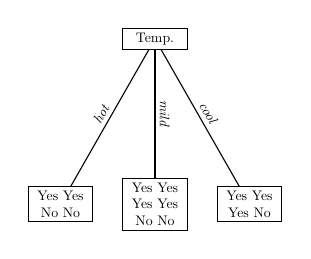
\begin{tikzpicture}[
		scale=0.6,
		every node/.style={scale=0.5},
		sloped
	]
		\node[bag]{\highlight{Temp.}}
		child {
			node[bag,align=center]{Yes Yes\\No No}
			edge from parent
			node[above]{\textit{hot}}
		}
    		child {
			node[bag,align=center]{Yes Yes\\Yes Yes\\No No}
			edge from parent
			node[above]{\textit{mild}}
		}
		child {
			node[bag,align=center]{Yes Yes\\Yes No}
			edge from parent
			node[above]{\textit{cool}}
		};
	\end{tikzpicture}
\end{figure}}